% 9 variables in here:
% h_1 = 10.0, h_2 = 12.0, h_3 = 10.0, ux_1 = 0.0, ux_2 = 0.0, ux_3 = 0.0, uy_1 = 0.0, uy_2 = 0.0, uy_3 = 0.0
\begin{figure}[h!]
\centering
  \subfigure[] {
    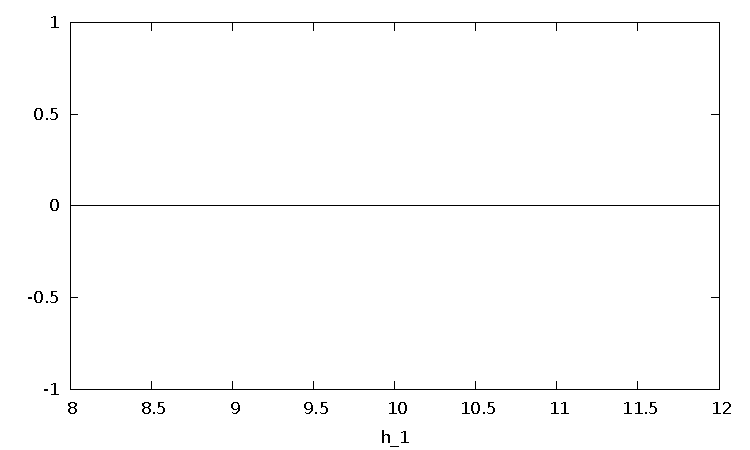
\includegraphics[scale=\zoomfactor]{{{slides_difference_1/y_12.0_10.0_0.0_0.0_0.0_0.0_0.0_0.0f00}}}
  }
  \subfigure[] {
    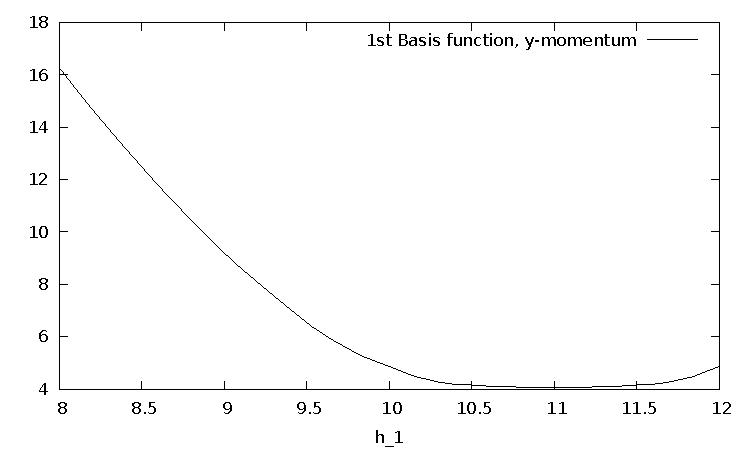
\includegraphics[scale=\zoomfactor]{{{slides_difference_1/y_12.0_10.0_0.0_0.0_0.0_0.0_0.0_0.0f01}}}
  }
  \subfigure[] {
    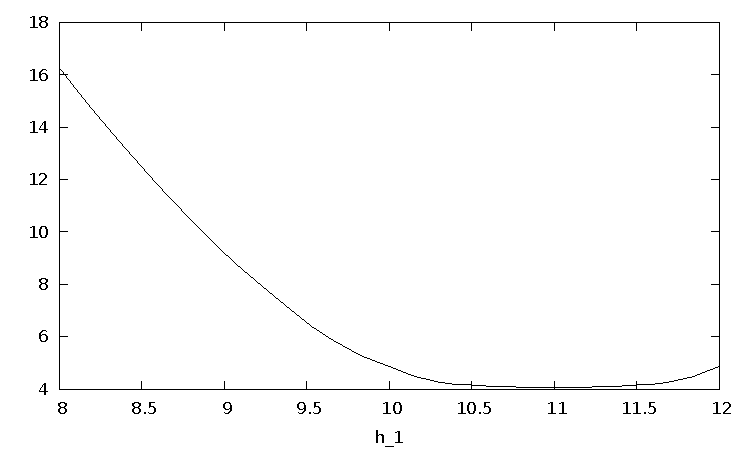
\includegraphics[scale=\zoomfactor]{{{slides_difference_1/y_12.0_10.0_0.0_0.0_0.0_0.0_0.0_0.0f02}}}
  }
  \subfigure[] {
    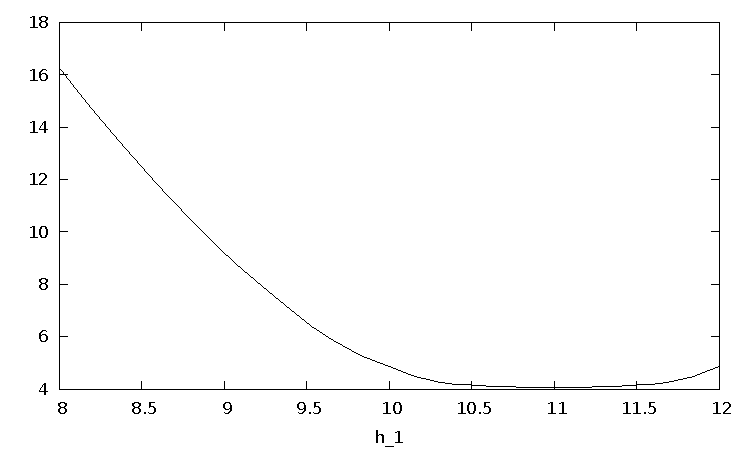
\includegraphics[scale=\zoomfactor]{{{slides_difference_1/y_12.0_10.0_0.0_0.0_0.0_0.0_0.0_0.0f03}}}
  }
  \subfigure[] {
    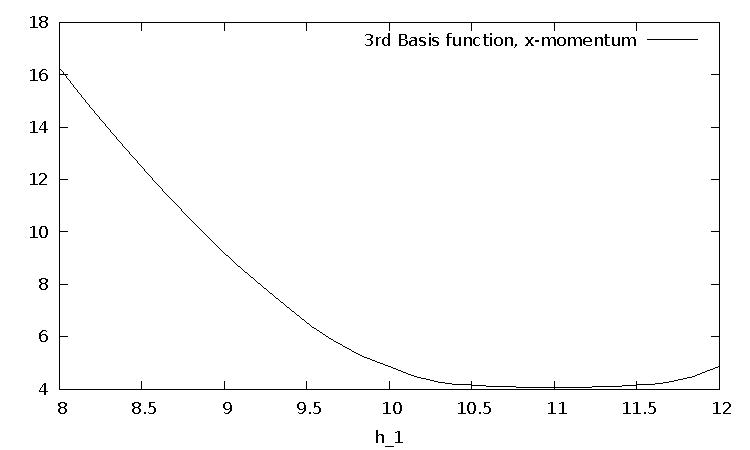
\includegraphics[scale=\zoomfactor]{{{slides_difference_1/y_12.0_10.0_0.0_0.0_0.0_0.0_0.0_0.0f04}}}
  }
  \subfigure[] {
    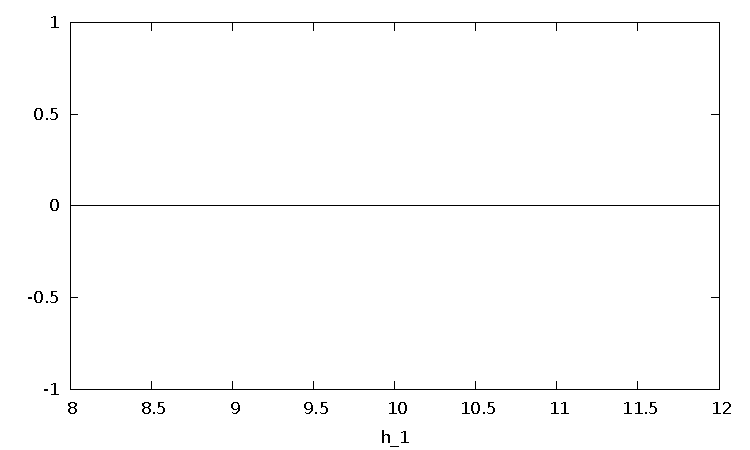
\includegraphics[scale=\zoomfactor]{{{slides_difference_1/y_12.0_10.0_0.0_0.0_0.0_0.0_0.0_0.0f05}}}
  }
\caption{}
\label{fig:slides_difference_1}
\end{figure}

%%% Local Variables:
%%% TeX-master: "../results.tex"
%%% End:
